\documentclass[]{article}
\usepackage{lmodern}
\usepackage{amssymb,amsmath}
\usepackage{ifxetex,ifluatex}
\usepackage{fixltx2e} % provides \textsubscript
\ifnum 0\ifxetex 1\fi\ifluatex 1\fi=0 % if pdftex
  \usepackage[T1]{fontenc}
  \usepackage[utf8]{inputenc}
\else % if luatex or xelatex
  \ifxetex
    \usepackage{mathspec}
    \usepackage{xltxtra,xunicode}
  \else
    \usepackage{fontspec}
  \fi
  \defaultfontfeatures{Mapping=tex-text,Scale=MatchLowercase}
  \newcommand{\euro}{€}
\fi
% use upquote if available, for straight quotes in verbatim environments
\IfFileExists{upquote.sty}{\usepackage{upquote}}{}
% use microtype if available
\IfFileExists{microtype.sty}{%
\usepackage{microtype}
\UseMicrotypeSet[protrusion]{basicmath} % disable protrusion for tt fonts
}{}
\usepackage[margin=1in]{geometry}
\usepackage{color}
\usepackage{fancyvrb}
\newcommand{\VerbBar}{|}
\newcommand{\VERB}{\Verb[commandchars=\\\{\}]}
\DefineVerbatimEnvironment{Highlighting}{Verbatim}{commandchars=\\\{\}}
% Add ',fontsize=\small' for more characters per line
\usepackage{framed}
\definecolor{shadecolor}{RGB}{248,248,248}
\newenvironment{Shaded}{\begin{snugshade}}{\end{snugshade}}
\newcommand{\KeywordTok}[1]{\textcolor[rgb]{0.13,0.29,0.53}{\textbf{{#1}}}}
\newcommand{\DataTypeTok}[1]{\textcolor[rgb]{0.13,0.29,0.53}{{#1}}}
\newcommand{\DecValTok}[1]{\textcolor[rgb]{0.00,0.00,0.81}{{#1}}}
\newcommand{\BaseNTok}[1]{\textcolor[rgb]{0.00,0.00,0.81}{{#1}}}
\newcommand{\FloatTok}[1]{\textcolor[rgb]{0.00,0.00,0.81}{{#1}}}
\newcommand{\CharTok}[1]{\textcolor[rgb]{0.31,0.60,0.02}{{#1}}}
\newcommand{\StringTok}[1]{\textcolor[rgb]{0.31,0.60,0.02}{{#1}}}
\newcommand{\CommentTok}[1]{\textcolor[rgb]{0.56,0.35,0.01}{\textit{{#1}}}}
\newcommand{\OtherTok}[1]{\textcolor[rgb]{0.56,0.35,0.01}{{#1}}}
\newcommand{\AlertTok}[1]{\textcolor[rgb]{0.94,0.16,0.16}{{#1}}}
\newcommand{\FunctionTok}[1]{\textcolor[rgb]{0.00,0.00,0.00}{{#1}}}
\newcommand{\RegionMarkerTok}[1]{{#1}}
\newcommand{\ErrorTok}[1]{\textbf{{#1}}}
\newcommand{\NormalTok}[1]{{#1}}
\usepackage{graphicx}
\makeatletter
\def\maxwidth{\ifdim\Gin@nat@width>\linewidth\linewidth\else\Gin@nat@width\fi}
\def\maxheight{\ifdim\Gin@nat@height>\textheight\textheight\else\Gin@nat@height\fi}
\makeatother
% Scale images if necessary, so that they will not overflow the page
% margins by default, and it is still possible to overwrite the defaults
% using explicit options in \includegraphics[width, height, ...]{}
\setkeys{Gin}{width=\maxwidth,height=\maxheight,keepaspectratio}
\ifxetex
  \usepackage[setpagesize=false, % page size defined by xetex
              unicode=false, % unicode breaks when used with xetex
              xetex]{hyperref}
\else
  \usepackage[unicode=true]{hyperref}
\fi
\hypersetup{breaklinks=true,
            bookmarks=true,
            pdfauthor={},
            pdftitle={},
            colorlinks=true,
            citecolor=blue,
            urlcolor=blue,
            linkcolor=magenta,
            pdfborder={0 0 0}}
\urlstyle{same}  % don't use monospace font for urls
\setlength{\parindent}{0pt}
\setlength{\parskip}{6pt plus 2pt minus 1pt}
\setlength{\emergencystretch}{3em}  % prevent overfull lines
\setcounter{secnumdepth}{0}

%%% Use protect on footnotes to avoid problems with footnotes in titles
\let\rmarkdownfootnote\footnote%
\def\footnote{\protect\rmarkdownfootnote}

%%% Change title format to be more compact
\usepackage{titling}

% Create subtitle command for use in maketitle
\newcommand{\subtitle}[1]{
  \posttitle{
    \begin{center}\large#1\end{center}
    }
}

\setlength{\droptitle}{-2em}
  \title{}
  \pretitle{\vspace{\droptitle}}
  \posttitle{}
  \author{}
  \preauthor{}\postauthor{}
  \date{}
  \predate{}\postdate{}



\begin{document}

\maketitle


\section{Reproducible Research}\label{reproducible-research}

\subsubsection{Peer Assessment 2:
PA2\_template}\label{peer-assessment-2-pa2ux5ftemplate}

\subsubsection{Introduction}\label{introduction}

This document presents the results of Peer Assessment 2 for the Coursera
course: Reproducible Research. This assessment required the student to
explore the NOAA Storm Database and answer some basic questions about
severe weather events.

The student must use the database to answer the questions below and show
code for your entire analysis. 1. Across the United States, which types
of events are most harmful with respect to population health? 2. Across
the United States, which types of events have the greatest economic
consequences?

\subsubsection{Data}\label{data}

This assignment makes use of data from the National Weather Service
Storm Database in the form of a comma-separated-value file compressed
via the bzip2 algorithm. The events in the database start in the year
1950 and end in November 2011. In the earlier years of the database
there are generally fewer events recorded, most likely due to a lack of
good records. More recent years should be considered more complete.

\begin{itemize}
\itemsep1pt\parskip0pt\parsep0pt
\item
  Dataset:
  \href{https://d396qusza40orc.cloudfront.net/repdata\%2Fdata\%2FStormData.csv.bz2}{storm
  data}
\end{itemize}

It consists of 902,297 observations on 37 variables.

\subsubsection{1. Loading Packages/ Data}\label{loading-packages-data}

\begin{Shaded}
\begin{Highlighting}[]
\NormalTok{for (package in }\KeywordTok{c}\NormalTok{(}\StringTok{'ggplot2'}\NormalTok{, }\StringTok{'dplyr'}\NormalTok{, }\StringTok{'gridExtra'}\NormalTok{)) \{}
 
    \NormalTok{if (!}\KeywordTok{require}\NormalTok{(package, }\DataTypeTok{character.only =} \OtherTok{TRUE}\NormalTok{, }\DataTypeTok{quietly =} \OtherTok{FALSE}\NormalTok{)) \{}
        \KeywordTok{install.packages}\NormalTok{(package)}
        \KeywordTok{library}\NormalTok{(package, }\DataTypeTok{character.only =} \OtherTok{TRUE}\NormalTok{)}
    \NormalTok{\}}
\NormalTok{\}}

\KeywordTok{remove}\NormalTok{(package)}

\NormalTok{val_dfpath <-}\StringTok{ }\KeywordTok{paste}\NormalTok{(}\KeywordTok{getwd}\NormalTok{(), }\StringTok{"data"}\NormalTok{, }\DataTypeTok{sep =} \StringTok{"/"}\NormalTok{)}
\NormalTok{val_dfname <-}\StringTok{ "repdata_data_StormData.csv.bz2"}
\NormalTok{val_dfdlink <-}\StringTok{ "http://d396qusza40orc.cloudfront.net/repdata%2Fdata%2FStormData.csv.bz2"}

\KeywordTok{tryCatch}\NormalTok{(\{}

  \NormalTok{if (}\KeywordTok{exists}\NormalTok{(}\StringTok{"data_storm.raw"}\NormalTok{) ==}\StringTok{ }\OtherTok{FALSE}\NormalTok{) \{}
 
    \NormalTok{if (}\KeywordTok{file.exists}\NormalTok{(}\KeywordTok{paste}\NormalTok{(val_dfpath, val_dfname, }\DataTypeTok{sep =} \StringTok{"/"}\NormalTok{)) ==}\StringTok{ }\OtherTok{FALSE}\NormalTok{) \{}
       
      \KeywordTok{dir.create}\NormalTok{(val_dfpath)}
      \KeywordTok{download.file}\NormalTok{(val_dfdlink, }\KeywordTok{paste}\NormalTok{(val_dfpath, val_dfname, }\DataTypeTok{sep =} \StringTok{"/"}\NormalTok{))}
       
    \NormalTok{\}}
     
    \NormalTok{temp_bzfile <-}\StringTok{ }\KeywordTok{bzfile}\NormalTok{(}\KeywordTok{paste}\NormalTok{(val_dfpath, val_dfname, }\DataTypeTok{sep =} \StringTok{"/"}\NormalTok{), }\StringTok{"r"}\NormalTok{)}
    \NormalTok{data_storm.raw <-}\StringTok{ }\KeywordTok{read.csv}\NormalTok{(temp_bzfile, }\DataTypeTok{stringsAsFactors =} \OtherTok{FALSE}\NormalTok{)}
 
  \NormalTok{\}}
      
\NormalTok{\}, }\DataTypeTok{error =} \NormalTok{function(e)\{}
      
  \KeywordTok{stop}\NormalTok{(}\StringTok{"Datafile error"}\NormalTok{)}
      
\NormalTok{\})}

\KeywordTok{remove}\NormalTok{(val_dfpath, val_dfname, val_dfdlink, temp_bzfile)}
\end{Highlighting}
\end{Shaded}

\subsubsection{2. Pre-process the Data}\label{pre-process-the-data}

Retrieve columns of interest:

\begin{Shaded}
\begin{Highlighting}[]
\NormalTok{val_stormcol <-}\StringTok{ }\KeywordTok{c}\NormalTok{(}\StringTok{"BGN_DATE"}\NormalTok{, }\StringTok{"EVTYPE"}\NormalTok{, }\StringTok{"FATALITIES"}\NormalTok{, }\StringTok{"INJURIES"}\NormalTok{,  }\StringTok{"PROPDMG"}\NormalTok{, }\StringTok{"PROPDMGEXP"}\NormalTok{, }\StringTok{"CROPDMG"}\NormalTok{, }\StringTok{"CROPDMGEXP"}\NormalTok{)}

\NormalTok{data_storm.sub <-}\StringTok{ }\NormalTok{data_storm.raw[, val_stormcol]}

\KeywordTok{remove}\NormalTok{(val_stormcol)}
\end{Highlighting}
\end{Shaded}

Group related `EVTYPE' records and store within new `SOURCE' column:

\begin{Shaded}
\begin{Highlighting}[]
\NormalTok{data_storm.sub$SOURCE <-}\StringTok{ }\OtherTok{NA}

\NormalTok{data_storm.sub[}\KeywordTok{grepl}\NormalTok{(}\StringTok{"precipitation|rain|hail|drizzle|wet|percip|burst|depression|fog|wall cloud"}\NormalTok{,}
  \NormalTok{data_storm.sub$EVTYPE, }\DataTypeTok{ignore.case =} \OtherTok{TRUE}\NormalTok{), }\StringTok{"SOURCE"}\NormalTok{] <-}\StringTok{ "Rain & Fog"}
\NormalTok{data_storm.sub[}\KeywordTok{grepl}\NormalTok{(}\StringTok{"storm|thunderstorm|lightning"}\NormalTok{,}
  \NormalTok{data_storm.sub$EVTYPE, }\DataTypeTok{ignore.case =} \OtherTok{TRUE}\NormalTok{), }\StringTok{"SOURCE"}\NormalTok{] <-}\StringTok{ "Storm"}
\NormalTok{data_storm.sub[}\KeywordTok{grepl}\NormalTok{(}\StringTok{"wind|wnd|hurricane|tornado|tstm|typhoon|spout|funnel|whirlwind"}\NormalTok{,}
  \NormalTok{data_storm.sub$EVTYPE, }\DataTypeTok{ignore.case =} \OtherTok{TRUE}\NormalTok{), }\StringTok{"SOURCE"}\NormalTok{] <-}\StringTok{ "Cyclone"}
\NormalTok{data_storm.sub[}\KeywordTok{grepl}\NormalTok{(}\StringTok{"slide|erosion|slump"}\NormalTok{,}
  \NormalTok{data_storm.sub$EVTYPE, }\DataTypeTok{ignore.case =} \OtherTok{TRUE}\NormalTok{), }\StringTok{"SOURCE"}\NormalTok{] <-}\StringTok{ "Landslide"}
\NormalTok{data_storm.sub[}\KeywordTok{grepl}\NormalTok{(}\StringTok{"warmth|warm|heat|dry|hot|drought|thermia|temperature record|record temperature|record high"}\NormalTok{,}
  \NormalTok{data_storm.sub$EVTYPE, }\DataTypeTok{ignore.case =} \OtherTok{TRUE}\NormalTok{), }\StringTok{"SOURCE"}\NormalTok{] <-}\StringTok{ "Extreme Heat"}
\NormalTok{data_storm.sub[}\KeywordTok{grepl}\NormalTok{(}\StringTok{"cold|cool|ice|icy|frost|freeze|snow|winter|wintry|wintery|blizzard|chill|freezing|avalanche|glaze|sleet"}\NormalTok{,}
  \NormalTok{data_storm.sub$EVTYPE, }\DataTypeTok{ignore.case =} \OtherTok{TRUE}\NormalTok{), }\StringTok{"SOURCE"}\NormalTok{] <-}\StringTok{ "Extreme Cold"}
\NormalTok{data_storm.sub[}\KeywordTok{grepl}\NormalTok{(}\StringTok{"flood|surf|blow-out|swells|fld|dam break|seas|high water|tide|tsunami|wave|current|marine|drowning"}\NormalTok{,}
  \NormalTok{data_storm.sub$EVTYPE, }\DataTypeTok{ignore.case =} \OtherTok{TRUE}\NormalTok{), }\StringTok{"SOURCE"}\NormalTok{] <-}\StringTok{ "Flood"}
\NormalTok{data_storm.sub[}\KeywordTok{grepl}\NormalTok{(}\StringTok{"dust|saharan"}\NormalTok{,}
  \NormalTok{data_storm.sub$EVTYPE, }\DataTypeTok{ignore.case =} \OtherTok{TRUE}\NormalTok{), }\StringTok{"SOURCE"}\NormalTok{] <-}\StringTok{ "Dust"}
\NormalTok{data_storm.sub[}\KeywordTok{grepl}\NormalTok{(}\StringTok{"fire|smoke|volcanic"}\NormalTok{,}
  \NormalTok{data_storm.sub$EVTYPE, }\DataTypeTok{ignore.case =} \OtherTok{TRUE}\NormalTok{), }\StringTok{"SOURCE"}\NormalTok{] <-}\StringTok{ "Fire & Smoke"}

\NormalTok{data_storm.sub$SOURCE[}\KeywordTok{is.na}\NormalTok{(data_storm.sub$SOURCE)] <-}\StringTok{ "Other"}

\NormalTok{##data_storm.sub <- group_by(data_storm.sub, SOURCE)}
\end{Highlighting}
\end{Shaded}

Derive total property and crop damage expense:

\begin{Shaded}
\begin{Highlighting}[]
\NormalTok{data_storm.sub$PROPDMGMULT <-}\StringTok{ }\OtherTok{NA}

\NormalTok{data_storm.sub[}\KeywordTok{grepl}\NormalTok{(}\StringTok{""}\NormalTok{,}
  \NormalTok{data_storm.sub$PROPDMGEXP, }\DataTypeTok{ignore.case =} \OtherTok{TRUE}\NormalTok{), }\StringTok{"PROPDMGMULT"}\NormalTok{] <-}\StringTok{ }\DecValTok{0}
\NormalTok{data_storm.sub[}\KeywordTok{grepl}\NormalTok{(}\StringTok{"H"}\NormalTok{,}
  \NormalTok{data_storm.sub$PROPDMGEXP, }\DataTypeTok{ignore.case =} \OtherTok{TRUE}\NormalTok{), }\StringTok{"PROPDMGMULT"}\NormalTok{] <-}\StringTok{ }\DecValTok{100}
\NormalTok{data_storm.sub[}\KeywordTok{grepl}\NormalTok{(}\StringTok{"K"}\NormalTok{,}
  \NormalTok{data_storm.sub$PROPDMGEXP, }\DataTypeTok{ignore.case =} \OtherTok{TRUE}\NormalTok{), }\StringTok{"PROPDMGMULT"}\NormalTok{] <-}\StringTok{ }\DecValTok{1000}
\NormalTok{data_storm.sub[}\KeywordTok{grepl}\NormalTok{(}\StringTok{"M"}\NormalTok{,}
  \NormalTok{data_storm.sub$PROPDMGEXP, }\DataTypeTok{ignore.case =} \OtherTok{TRUE}\NormalTok{), }\StringTok{"PROPDMGMULT"}\NormalTok{] <-}\StringTok{ }\DecValTok{1000000}
\NormalTok{data_storm.sub[}\KeywordTok{grepl}\NormalTok{(}\StringTok{"B"}\NormalTok{,}
  \NormalTok{data_storm.sub$PROPDMGEXP, }\DataTypeTok{ignore.case =} \OtherTok{TRUE}\NormalTok{), }\StringTok{"PROPDMGMULT"}\NormalTok{] <-}\StringTok{ }\DecValTok{1000000000}

\NormalTok{data_storm.sub$PROPDMGEXPMULT <-}\StringTok{ }\NormalTok{data_storm.sub$PROPDMG *}\StringTok{ }\NormalTok{data_storm.sub$PROPDMGMULT}

\NormalTok{data_storm.sub$CROPDMGMULT <-}\StringTok{ }\OtherTok{NA}

\NormalTok{data_storm.sub[}\KeywordTok{grepl}\NormalTok{(}\StringTok{""}\NormalTok{,}
  \NormalTok{data_storm.sub$CROPDMGEXP, }\DataTypeTok{ignore.case =} \OtherTok{TRUE}\NormalTok{), }\StringTok{"CROPDMGMULT"}\NormalTok{] <-}\StringTok{ }\DecValTok{0}
\NormalTok{data_storm.sub[}\KeywordTok{grepl}\NormalTok{(}\StringTok{"H"}\NormalTok{,}
  \NormalTok{data_storm.sub$CROPDMGEXP, }\DataTypeTok{ignore.case =} \OtherTok{TRUE}\NormalTok{), }\StringTok{"CROPDMGMULT"}\NormalTok{] <-}\StringTok{ }\DecValTok{100}
\NormalTok{data_storm.sub[}\KeywordTok{grepl}\NormalTok{(}\StringTok{"K"}\NormalTok{,}
  \NormalTok{data_storm.sub$CROPDMGEXP, }\DataTypeTok{ignore.case =} \OtherTok{TRUE}\NormalTok{), }\StringTok{"CROPDMGMULT"}\NormalTok{] <-}\StringTok{ }\DecValTok{1000}
\NormalTok{data_storm.sub[}\KeywordTok{grepl}\NormalTok{(}\StringTok{"M"}\NormalTok{,}
  \NormalTok{data_storm.sub$CROPDMGEXP, }\DataTypeTok{ignore.case =} \OtherTok{TRUE}\NormalTok{), }\StringTok{"CROPDMGMULT"}\NormalTok{] <-}\StringTok{ }\DecValTok{1000000}
\NormalTok{data_storm.sub[}\KeywordTok{grepl}\NormalTok{(}\StringTok{"B"}\NormalTok{,}
  \NormalTok{data_storm.sub$CROPDMGEXP, }\DataTypeTok{ignore.case =} \OtherTok{TRUE}\NormalTok{), }\StringTok{"CROPDMGMULT"}\NormalTok{] <-}\StringTok{ }\DecValTok{1000000000}

\NormalTok{data_storm.sub$CROPDMGEXPMULT <-}\StringTok{ }\NormalTok{data_storm.sub$CROPDMG *}\StringTok{ }\NormalTok{data_storm.sub$CROPDMGMULT}
\end{Highlighting}
\end{Shaded}

Combine `INJURIES' and `FATALITIES', as well as `PROPDMGEXP' and
`CROPDMGEXP':

\begin{Shaded}
\begin{Highlighting}[]
\NormalTok{data_storm.sub <-}\StringTok{ }\KeywordTok{mutate}\NormalTok{(data_storm.sub, }\DataTypeTok{CASUALTIES =} \NormalTok{INJURIES +}\StringTok{ }\NormalTok{FATALITIES)}
\NormalTok{data_storm.sub <-}\StringTok{ }\KeywordTok{mutate}\NormalTok{(data_storm.sub, }\DataTypeTok{DMGEXPMULT =} \NormalTok{PROPDMGEXPMULT +}\StringTok{ }\NormalTok{CROPDMGEXPMULT)}
\end{Highlighting}
\end{Shaded}

Identify records by year and subset pre/post-1990 data (hidden due to
assessment plot limit):

\begin{Shaded}
\begin{Highlighting}[]
\NormalTok{data_storm.sub <-}\StringTok{ }\KeywordTok{data.frame}\NormalTok{(data_storm.sub[}\DecValTok{1}\NormalTok{],}
  \DataTypeTok{YEAR =} \KeywordTok{as.numeric}\NormalTok{(}\KeywordTok{format}\NormalTok{(}\KeywordTok{as.Date}\NormalTok{(data_storm.sub[, }\DecValTok{1}\NormalTok{], }\DataTypeTok{format =} \StringTok{"%m/%d/%Y %H:%M:%S"}\NormalTok{), }\StringTok{"%Y"}\NormalTok{)),}
  \NormalTok{data_storm.sub[}\DecValTok{2}\NormalTok{:}\KeywordTok{ncol}\NormalTok{(data_storm.sub)])}

\NormalTok{val_recordbyyear <-}\StringTok{ }\KeywordTok{ggplot}\NormalTok{(}\DataTypeTok{data =} \NormalTok{data_storm.sub, }\KeywordTok{aes}\NormalTok{(}\DataTypeTok{x =} \NormalTok{YEAR)) +}
\StringTok{  }\KeywordTok{geom_histogram}\NormalTok{(}\DataTypeTok{binwidth =} \FloatTok{0.1}\NormalTok{, }\DataTypeTok{col =} \StringTok{"black"}\NormalTok{, }\DataTypeTok{alpha =} \FloatTok{0.5}\NormalTok{) +}
\StringTok{  }\KeywordTok{geom_vline}\NormalTok{(}\DataTypeTok{xintercept =} \DecValTok{1990}\NormalTok{, }\DataTypeTok{color =} \StringTok{"red"}\NormalTok{) +}
\StringTok{  }\KeywordTok{ggtitle}\NormalTok{(}\StringTok{"Figure x: Observations by Year"}\NormalTok{)}
  
\NormalTok{data_storm.sub.inc1 <-}\StringTok{ }\NormalTok{data_storm.sub[data_storm.sub$YEAR <}\StringTok{ }\DecValTok{1990}\NormalTok{, ]}
\NormalTok{data_storm.sub.inc2 <-}\StringTok{ }\NormalTok{data_storm.sub[data_storm.sub$YEAR >=}\StringTok{ }\DecValTok{1990}\NormalTok{, ]}
\end{Highlighting}
\end{Shaded}

\subsubsection{3. Exploratory Data
Analysis}\label{exploratory-data-analysis}

Conduct summary statistics on `INJURIES' and `FATALITIES', store in new
dataframe:

\begin{Shaded}
\begin{Highlighting}[]
\NormalTok{data_storm.sum1.inc1 <-}\StringTok{ }\KeywordTok{aggregate}\NormalTok{(INJURIES ~}\StringTok{ }\NormalTok{SOURCE, }\DataTypeTok{data =} \NormalTok{data_storm.sub.inc1, }\DataTypeTok{FUN =} \NormalTok{sum)}
\NormalTok{data_storm.sum1.inc2 <-}\StringTok{ }\KeywordTok{aggregate}\NormalTok{(INJURIES ~}\StringTok{ }\NormalTok{SOURCE, }\DataTypeTok{data =} \NormalTok{data_storm.sub.inc2, }\DataTypeTok{FUN =} \NormalTok{sum)}

\NormalTok{data_storm.sum2.inc1 <-}\StringTok{ }\KeywordTok{aggregate}\NormalTok{(FATALITIES ~}\StringTok{ }\NormalTok{SOURCE, }\DataTypeTok{data =} \NormalTok{data_storm.sub.inc1, }\DataTypeTok{FUN =} \NormalTok{sum)}
\NormalTok{data_storm.sum2.inc2 <-}\StringTok{ }\KeywordTok{aggregate}\NormalTok{(FATALITIES ~}\StringTok{ }\NormalTok{SOURCE, }\DataTypeTok{data =} \NormalTok{data_storm.sub.inc2, }\DataTypeTok{FUN =} \NormalTok{sum)}

\NormalTok{data_storm.sum1.inc1 <-}\StringTok{ }\KeywordTok{arrange}\NormalTok{(data_storm.sum1.inc1, -INJURIES)}
\NormalTok{data_storm.sum1.inc2 <-}\StringTok{ }\KeywordTok{arrange}\NormalTok{(data_storm.sum1.inc2, -INJURIES)}

\NormalTok{data_storm.sum2.inc1 <-}\StringTok{ }\KeywordTok{arrange}\NormalTok{(data_storm.sum2.inc1, -FATALITIES)}
\NormalTok{data_storm.sum2.inc2 <-}\StringTok{ }\KeywordTok{arrange}\NormalTok{(data_storm.sum2.inc2, -FATALITIES)}
\end{Highlighting}
\end{Shaded}

Plot post-1990, injury/fatality data:

\begin{Shaded}
\begin{Highlighting}[]
\NormalTok{val_storminc2plot1  <-}\StringTok{ }\KeywordTok{ggplot}\NormalTok{(data_storm.sum1.inc2, }\KeywordTok{aes}\NormalTok{(}\DataTypeTok{x =} \KeywordTok{reorder}\NormalTok{(SOURCE, INJURIES), }\DataTypeTok{y =} \NormalTok{INJURIES)) +}
\StringTok{  }\KeywordTok{geom_bar}\NormalTok{(}\DataTypeTok{stat =} \StringTok{"identity"}\NormalTok{, }\DataTypeTok{fill =} \StringTok{"red"}\NormalTok{, }\DataTypeTok{alpha =} \FloatTok{0.5}\NormalTok{) +}
\StringTok{  }\KeywordTok{coord_flip}\NormalTok{() +}
\StringTok{  }\KeywordTok{ggtitle}\NormalTok{(}\StringTok{"Figure 1a: Total Injuries by Severe Weather - Post-1990"}\NormalTok{) +}
\StringTok{  }\KeywordTok{theme}\NormalTok{(}\DataTypeTok{axis.title.y =} \KeywordTok{element_blank}\NormalTok{())}

\NormalTok{val_storminc2plot2  <-}\StringTok{ }\KeywordTok{ggplot}\NormalTok{(data_storm.sum2.inc2, }\KeywordTok{aes}\NormalTok{(}\DataTypeTok{x =} \KeywordTok{reorder}\NormalTok{(SOURCE, FATALITIES), }\DataTypeTok{y =} \NormalTok{FATALITIES)) +}
\StringTok{  }\KeywordTok{geom_bar}\NormalTok{(}\DataTypeTok{stat =} \StringTok{"identity"}\NormalTok{, }\DataTypeTok{fill =} \StringTok{"red"}\NormalTok{, }\DataTypeTok{alpha =} \FloatTok{0.5}\NormalTok{) +}
\StringTok{  }\KeywordTok{coord_flip}\NormalTok{() +}
\StringTok{  }\KeywordTok{ggtitle}\NormalTok{(}\StringTok{"Figure 1b: Total Fatalities by Severe Weather - Post-1990"}\NormalTok{) +}
\StringTok{  }\KeywordTok{theme}\NormalTok{(}\DataTypeTok{axis.title.y =} \KeywordTok{element_blank}\NormalTok{())}

\KeywordTok{grid.arrange}\NormalTok{(val_storminc2plot1, val_storminc2plot2, }\DataTypeTok{ncol =} \DecValTok{2}\NormalTok{)}
\end{Highlighting}
\end{Shaded}

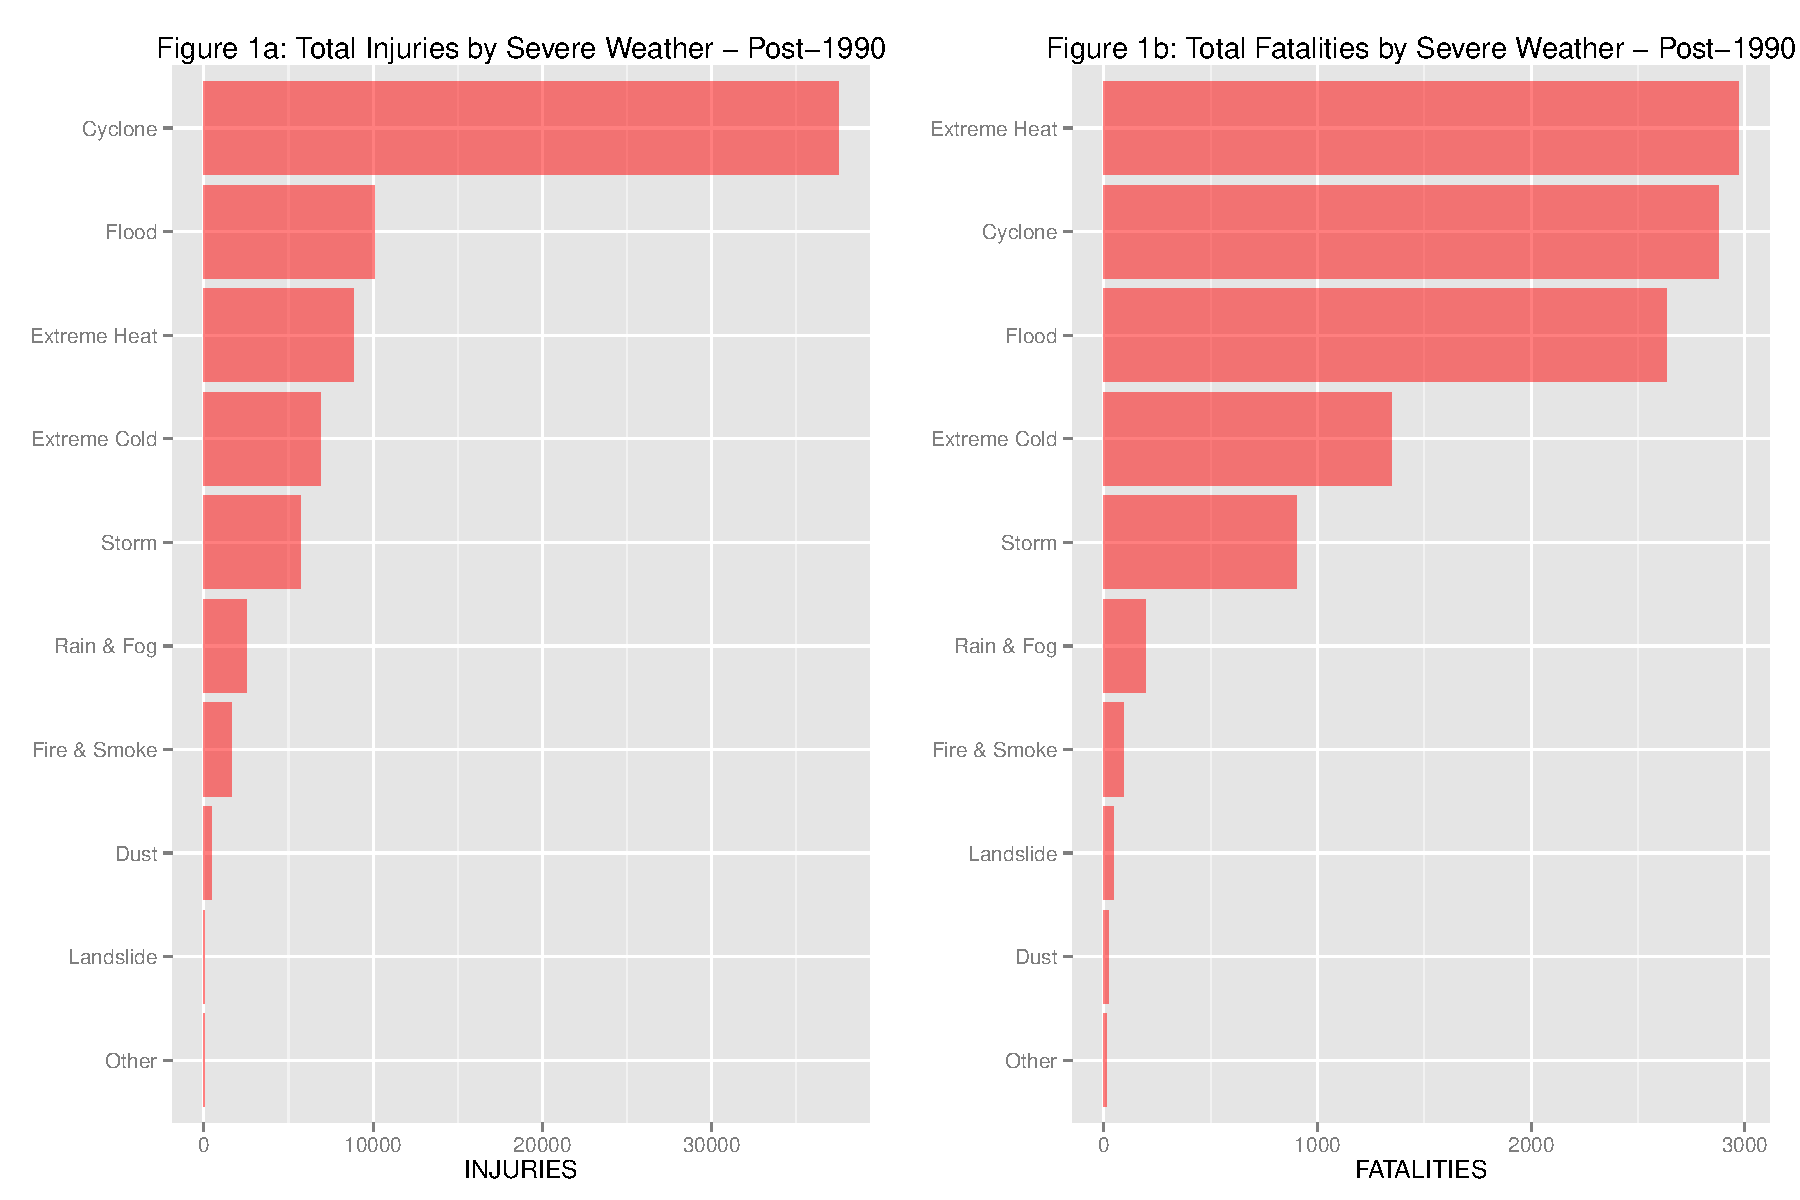
\includegraphics{figure/unnamed-chunk-8-1.pdf} Plot shows that `Cyclone'
category events have caused the most injuries post-1990. `Extreme Heat'
events have caused the most fatalities post-1990.

Conduct summary statistics on cyclone related `CASUALTIES' and store in
new dataframe:

\begin{Shaded}
\begin{Highlighting}[]
\NormalTok{data_storm.sub.inc2.cyc <-}\StringTok{ }\NormalTok{data_storm.sub.inc2[}\KeywordTok{grep}\NormalTok{(}\StringTok{"Cyclone"}\NormalTok{, data_storm.sub.inc2$SOURCE, }\DataTypeTok{perl =} \OtherTok{TRUE}\NormalTok{), ]}

\NormalTok{data_storm.sum.inc2.cyc <-}\StringTok{ }\KeywordTok{aggregate}\NormalTok{(CASUALTIES ~}\StringTok{ }\NormalTok{EVTYPE, }\DataTypeTok{data =} \NormalTok{data_storm.sub.inc2.cyc, }\DataTypeTok{FUN =} \NormalTok{sum)}

\NormalTok{data_storm.sum.inc2.cyc <-}\StringTok{ }\KeywordTok{arrange}\NormalTok{(data_storm.sum.inc2.cyc, -CASUALTIES)}

\NormalTok{data_storm.sum.inc2.cyc <-}\StringTok{ }\KeywordTok{head}\NormalTok{(data_storm.sum.inc2.cyc, }\DecValTok{10}\NormalTok{)}
\end{Highlighting}
\end{Shaded}

Plot post-1990 tornado related `CASUALTIES' (hidden due to assessment
plot limit):

\begin{Shaded}
\begin{Highlighting}[]
\NormalTok{val_post90casualties <-}\StringTok{ }\KeywordTok{ggplot}\NormalTok{(data_storm.sum.inc2.cyc, }\KeywordTok{aes}\NormalTok{(}\DataTypeTok{x =} \KeywordTok{reorder}\NormalTok{(EVTYPE, CASUALTIES), }\DataTypeTok{y =} \NormalTok{CASUALTIES)) +}
\StringTok{  }\KeywordTok{geom_bar}\NormalTok{(}\DataTypeTok{stat =} \StringTok{"identity"}\NormalTok{, }\DataTypeTok{fill =} \StringTok{"red"}\NormalTok{, }\DataTypeTok{alpha =} \FloatTok{0.5}\NormalTok{) +}
\StringTok{  }\KeywordTok{coord_flip}\NormalTok{() +}
\StringTok{  }\KeywordTok{ggtitle}\NormalTok{(}\StringTok{"Figure x: Total Tornado Related Casualties - Post-1990"}\NormalTok{) +}
\StringTok{  }\KeywordTok{theme}\NormalTok{(}\DataTypeTok{axis.title.y =} \KeywordTok{element_blank}\NormalTok{())}
\end{Highlighting}
\end{Shaded}

Conduct summary statistics on `PROPDMGEXP' and `CROPDMGEXP', store in
new dataframe:

\begin{Shaded}
\begin{Highlighting}[]
\NormalTok{data_storm.sum3.inc1 <-}\StringTok{ }\KeywordTok{aggregate}\NormalTok{(PROPDMGEXPMULT ~}\StringTok{ }\NormalTok{SOURCE, }\DataTypeTok{data =} \NormalTok{data_storm.sub.inc1, }\DataTypeTok{FUN =} \NormalTok{sum)}
\NormalTok{data_storm.sum3.inc2 <-}\StringTok{ }\KeywordTok{aggregate}\NormalTok{(PROPDMGEXPMULT ~}\StringTok{ }\NormalTok{SOURCE, }\DataTypeTok{data =} \NormalTok{data_storm.sub.inc2, }\DataTypeTok{FUN =} \NormalTok{sum)}

\NormalTok{data_storm.sum4.inc1 <-}\StringTok{ }\KeywordTok{aggregate}\NormalTok{(CROPDMGEXPMULT ~}\StringTok{ }\NormalTok{SOURCE, }\DataTypeTok{data =} \NormalTok{data_storm.sub.inc1, }\DataTypeTok{FUN =} \NormalTok{sum)}
\NormalTok{data_storm.sum4.inc2 <-}\StringTok{ }\KeywordTok{aggregate}\NormalTok{(CROPDMGEXPMULT ~}\StringTok{ }\NormalTok{SOURCE, }\DataTypeTok{data =} \NormalTok{data_storm.sub.inc2, }\DataTypeTok{FUN =} \NormalTok{sum)}

\NormalTok{data_storm.sum3.inc1 <-}\StringTok{ }\KeywordTok{arrange}\NormalTok{(data_storm.sum3.inc1, -PROPDMGEXPMULT)}
\NormalTok{data_storm.sum3.inc2 <-}\StringTok{ }\KeywordTok{arrange}\NormalTok{(data_storm.sum3.inc2, -PROPDMGEXPMULT)}

\NormalTok{data_storm.sum4.inc1 <-}\StringTok{ }\KeywordTok{arrange}\NormalTok{(data_storm.sum4.inc1, -CROPDMGEXPMULT)}
\NormalTok{data_storm.sum4.inc2 <-}\StringTok{ }\KeywordTok{arrange}\NormalTok{(data_storm.sum4.inc2, -CROPDMGEXPMULT)}
\end{Highlighting}
\end{Shaded}

Plot post-1990, property/crop damage expense data:

\begin{Shaded}
\begin{Highlighting}[]
\NormalTok{val_storminc2plot1  <-}\StringTok{ }\KeywordTok{ggplot}\NormalTok{(data_storm.sum3.inc2, }\KeywordTok{aes}\NormalTok{(}\DataTypeTok{x =} \KeywordTok{reorder}\NormalTok{(SOURCE, PROPDMGEXPMULT), }\DataTypeTok{y =} \NormalTok{PROPDMGEXPMULT)) +}
\StringTok{  }\KeywordTok{geom_bar}\NormalTok{(}\DataTypeTok{stat =} \StringTok{"identity"}\NormalTok{, }\DataTypeTok{fill =} \StringTok{"blue"}\NormalTok{, }\DataTypeTok{alpha =} \FloatTok{0.5}\NormalTok{) +}
\StringTok{  }\KeywordTok{coord_flip}\NormalTok{() +}
\StringTok{  }\KeywordTok{ggtitle}\NormalTok{(}\StringTok{"Figure 2a: Total Property Damage by Severe Weather - Post-1990"}\NormalTok{) +}
\StringTok{  }\KeywordTok{theme}\NormalTok{(}\DataTypeTok{axis.title.y =} \KeywordTok{element_blank}\NormalTok{())}

\NormalTok{val_storminc2plot2  <-}\StringTok{ }\KeywordTok{ggplot}\NormalTok{(data_storm.sum4.inc2, }\KeywordTok{aes}\NormalTok{(}\DataTypeTok{x =} \KeywordTok{reorder}\NormalTok{(SOURCE, CROPDMGEXPMULT), }\DataTypeTok{y =} \NormalTok{CROPDMGEXPMULT)) +}
\StringTok{  }\KeywordTok{geom_bar}\NormalTok{(}\DataTypeTok{stat =} \StringTok{"identity"}\NormalTok{, }\DataTypeTok{fill =} \StringTok{"blue"}\NormalTok{, }\DataTypeTok{alpha =} \FloatTok{0.5}\NormalTok{) +}
\StringTok{  }\KeywordTok{coord_flip}\NormalTok{() +}
\StringTok{  }\KeywordTok{ggtitle}\NormalTok{(}\StringTok{"Figure 2b: Total Crop Damage by Severe Weather - Post-1990"}\NormalTok{) +}
\StringTok{  }\KeywordTok{theme}\NormalTok{(}\DataTypeTok{axis.title.y =} \KeywordTok{element_blank}\NormalTok{())}

\KeywordTok{grid.arrange}\NormalTok{(val_storminc2plot1, val_storminc2plot2, }\DataTypeTok{ncol =} \DecValTok{2}\NormalTok{)}
\end{Highlighting}
\end{Shaded}

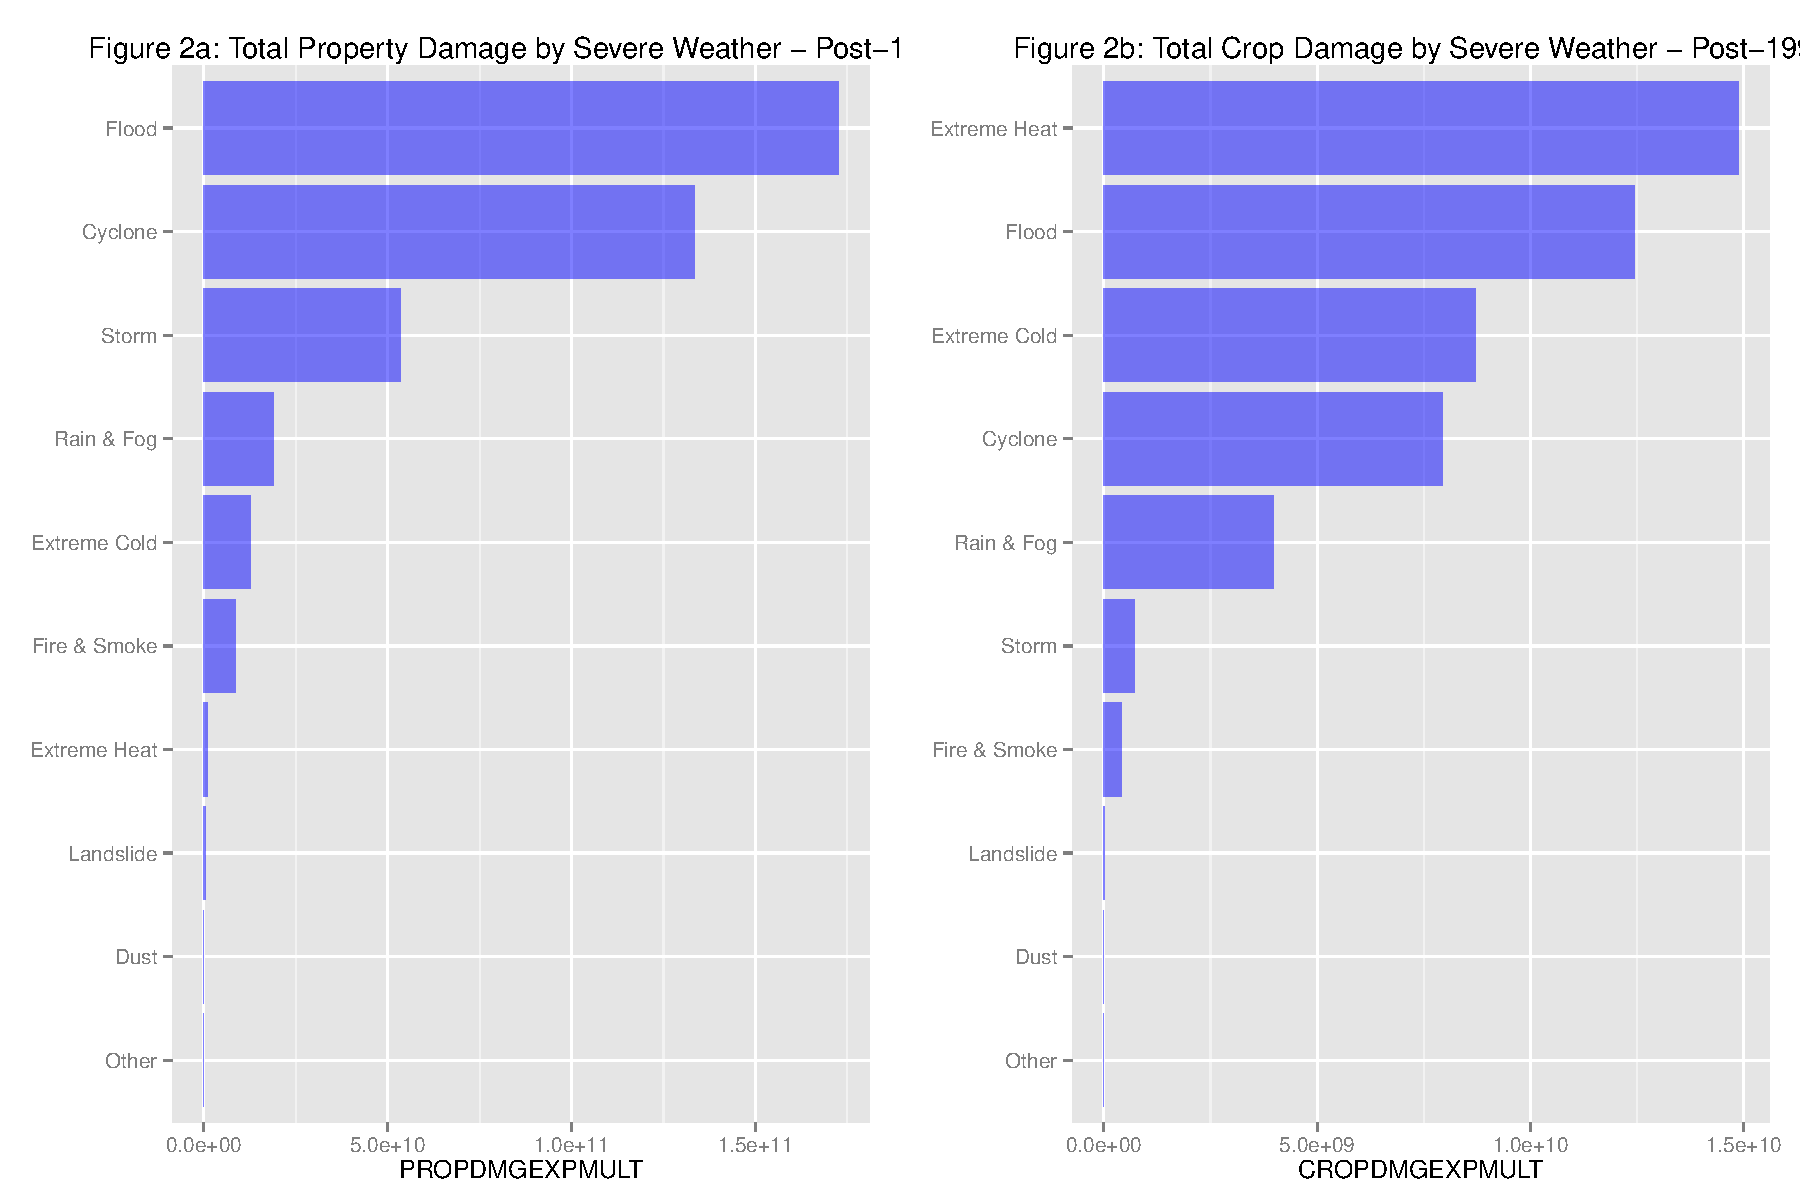
\includegraphics{figure/unnamed-chunk-12-1.pdf} Plot shows that `Flood'
category events have caused the most property damage post-1990. `Extreme
Heat' events have caused the most crop damage post-1990.

Conduct summary statistics on `DMGEXP' and store in new dataframe:

\begin{Shaded}
\begin{Highlighting}[]
\NormalTok{data_storm.sub.inc2.flood <-}\StringTok{ }\NormalTok{data_storm.sub.inc2[}\KeywordTok{grep}\NormalTok{(}\StringTok{"Flood"}\NormalTok{, data_storm.sub.inc2$SOURCE, }\DataTypeTok{perl =} \OtherTok{TRUE}\NormalTok{), ]}

\NormalTok{data_storm.sum.inc2.flood <-}\StringTok{ }\KeywordTok{aggregate}\NormalTok{(DMGEXPMULT ~}\StringTok{ }\NormalTok{EVTYPE, }\DataTypeTok{data =} \NormalTok{data_storm.sub.inc2.flood, }\DataTypeTok{FUN =} \NormalTok{sum)}

\NormalTok{data_storm.sum.inc2.flood <-}\StringTok{ }\KeywordTok{arrange}\NormalTok{(data_storm.sum.inc2.flood, -DMGEXPMULT)}

\NormalTok{data_storm.sum.inc2.flood <-}\StringTok{ }\KeywordTok{head}\NormalTok{(data_storm.sum.inc2.flood, }\DecValTok{10}\NormalTok{)}
\end{Highlighting}
\end{Shaded}

Plot post-1990 flood related `DMGEXP' (hidden due to assessment plot
limit):

\begin{Shaded}
\begin{Highlighting}[]
\NormalTok{val_post90flood <-}\StringTok{ }\KeywordTok{ggplot}\NormalTok{(data_storm.sum.inc2.flood, }\KeywordTok{aes}\NormalTok{(}\DataTypeTok{x =} \KeywordTok{reorder}\NormalTok{(EVTYPE, DMGEXPMULT), }\DataTypeTok{y =} \NormalTok{DMGEXPMULT)) +}
\StringTok{  }\KeywordTok{geom_bar}\NormalTok{(}\DataTypeTok{stat =} \StringTok{"identity"}\NormalTok{, }\DataTypeTok{fill =} \StringTok{"blue"}\NormalTok{, }\DataTypeTok{alpha =} \FloatTok{0.5}\NormalTok{) +}
\StringTok{  }\KeywordTok{coord_flip}\NormalTok{() +}
\StringTok{  }\KeywordTok{ggtitle}\NormalTok{(}\StringTok{"Figure x: Total Damage by Severe Weather - Post-1990"}\NormalTok{) +}
\StringTok{  }\KeywordTok{theme}\NormalTok{(}\DataTypeTok{axis.title.y =} \KeywordTok{element_blank}\NormalTok{())}
\end{Highlighting}
\end{Shaded}

\end{document}
